\documentclass[a4paper]{article}
\def\DOCTITLE{CSC8502 Advanced Graphics for Games}
% Set document attributes
\title{\DOCTITLE}

\usepackage{fullpage}
\usepackage{scrextend}
\usepackage{titlesec}
\usepackage{fancyhdr}
\usepackage{amsmath}
\usepackage{amssymb}
\usepackage[section]{placeins}
\usepackage{booktabs}
\usepackage{hyperref}
\usepackage{tikz}
\usepackage{graphicx}
\usepackage{minted}
\usepackage{subcaption}

% Setup headers and footers
\pagestyle{fancy}
\lhead{}
\chead{\DOCTITLE}
\rhead{}
\rfoot{}
\cfoot{\thepage}
\lfoot{}

% New page for each section
\newcommand{\sectionbreak}{\clearpage}

% Set header and footer sizes
\renewcommand{\headrulewidth}{0.4pt}
\renewcommand{\footrulewidth}{0.4pt}
\setlength{\headheight}{15.2pt}
\setlength{\headsep}{15.2pt}

\setlength{\parskip}{5pt plus 1pt minus 1pt}
\setlength{\parindent}{0pt}

% Newline after paragraph
\newcommand{\Para}[1]{\paragraph{#1}\mbox{}}

% Stuff used in cryptography notes
\newcommand{\Forall}{\;\forall\;}
\newcommand{\Mod}{\: mod \:}

% Stuff used in distributed systems notes
\newcommand{\happenbefore}{\rightarrow}
\newcommand{\orderbefore}{\Rightarrow}
\newcommand{\clockcond}{\leadsto}
\newcommand{\RArrow}{$\rightarrow$}

\def\checkmark{\tikz\fill[scale=0.4](0,.35) -- (.25,0) -- (1,.7) -- (.25,.15) -- cycle;}


\begin{document}

\tableofcontents

\vfill
Course material:
\url{https://research.ncl.ac.uk/game/mastersdegree/graphicsforgames/}

\section{Overview}

\subsection{3D Graphics}

\begin{itemize}
  \item Scene made up of objects made up of primitives
  \item Primitives are a collection of vertices
  \item Vertices have attributes (position, colour, texture coordinate, etc.)
\end{itemize}

\subsubsection{Primitives}

\begin{figure}[h]
  \centering

  \begin{subfigure}[b]{0.3\textwidth}
    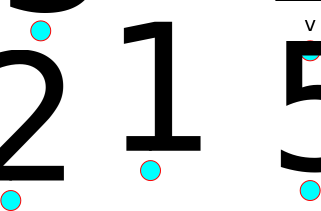
\includegraphics[width=0.8\textwidth]{out/rast_pri_points.eps}
    \caption{Point}
  \end{subfigure}
  \begin{subfigure}[b]{0.3\textwidth}
    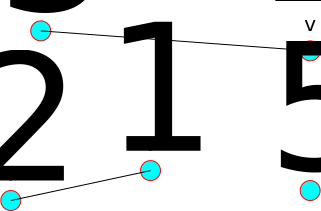
\includegraphics[width=0.8\textwidth]{out/rast_pri_lines.eps}
    \caption{Line}
  \end{subfigure}
  \begin{subfigure}[b]{0.3\textwidth}
    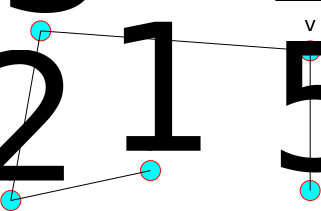
\includegraphics[width=0.8\textwidth]{out/rast_pri_line_strip.eps}
    \caption{Line Strip}
  \end{subfigure}

  \vspace{2em}

  \begin{subfigure}[b]{0.3\textwidth}
    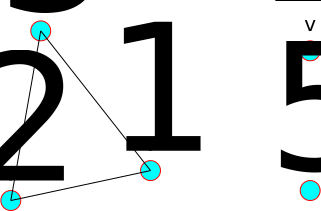
\includegraphics[width=0.8\textwidth]{out/rast_pri_triangle.eps}
    \caption{Triangle}
  \end{subfigure}
  \begin{subfigure}[b]{0.3\textwidth}
    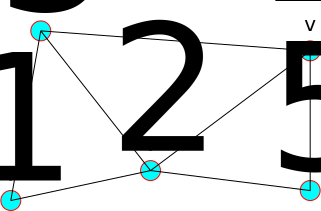
\includegraphics[width=0.8\textwidth]{out/rast_pri_triangle_strip.eps}
    \caption{Triangle Strip}
  \end{subfigure}
  \begin{subfigure}[b]{0.3\textwidth}
    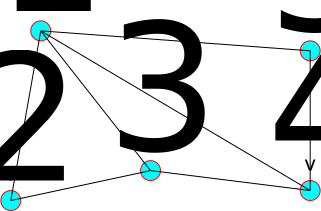
\includegraphics[width=0.8\textwidth]{out/rast_pri_triangle_fan.eps}
    \caption{Triangle Fan}
  \end{subfigure}

  \caption{}
  \label{fig:primitives}
\end{figure}
\FloatBarrier

\subsection{Graphics Pipeline}

\begin{figure}[h!]
  \centering
  TODO: use new diagran
  % \includegraphics[width=0.6\textwidth]{out/graphic_pipeline.eps}
  \caption{OpenGL Pipeline}
  \label{fig:graphics_pipeline}
\end{figure}
\FloatBarrier

\subsection{OpenGL}

Useful (somewhat) OpenGL related stuff to know:

\begin{itemize}
  \item
    Buffers
    \begin{itemize}
      \item
        OpenGL buffers are generated from data in main memory

      \item
        Buffer generation copies data to graphics memory

      \item
        Data in main memory is no longer required

      \item
        OpenGL buffers can be bound to CPU memory addresses to modify buffer
        contents

    \end{itemize}

  \item
    Shaders
    \begin{itemize}
      \item
        Operate per item (per vertex for vertex and tessellation shaders, per
        primitive for geometry shader, per fragment for fragment shader)

      \item
        Data common to all shaders passed as uniforms

    \end{itemize}
\end{itemize}

\section{Transformations}
\label{sec:transformations}

\subsection{Spaces}

\begin{description}
  \item[World] \hfill \\
    3D space containing everything

  \item[Camera] \hfill \\
    3D space containing the view from the camera \\
    Origin is camera position \\
    Obtained through camera transform

  \item[Clip] \hfill \\
    Only the primitives that can be seen by the camera \\
    Obtained through perspective transform

  \item[Normalised Device Coordinates] \hfill \\
    Transformed from clip space \\
    Coordinates normalised to 1 for hardware compatibility

  \item[Viewport Coordinates] \hfill \\
    Coordinates on a particular screen

\end{description}

\subsection{Scale}

Scale matrix to scale by $x$, $y$ and $z$ is each respective axis:
\[
  \left [
    \begin{array}{cccc}
      x & 0 & 0 & 0 \\
      0 & y & 0 & 0 \\
      0 & 0 & z & 0 \\
      0 & 0 & 0 & 1
    \end{array}
  \right ]
\]

\subsection{Translation}

Translation matrix to move by $x$, $y$ and $z$ is each respective axis:
\[
  \left [
    \begin{array}{cccc}
      1 & 0 & 0 & x \\
      0 & 1 & 0 & y \\
      0 & 0 & 1 & z \\
      0 & 0 & 0 & 1
    \end{array}
  \right ]
\]

\subsection{Rotation}

Rotation about $x$ axis by $\theta$:
\[
  \left [
    \begin{array}{cccc}
      1 & 0           & 0         & 0 \\
      0 & cos\theta   & sin\theta & 0 \\
      0 & -sin\theta  & cos\theta & 0 \\
      0 & 0           & 0         & 1
    \end{array}
  \right ]
\]

Rotation about $y$ axis by $\theta$:
\[
  \left [
    \begin{array}{cccc}
      cos\theta   & 0 & sin\theta & 0 \\
      0           & 1 & 0         & 0 \\
      -sin\theta  & 0 & cos\theta & 0 \\
      0           & 0 & 0         & 1
    \end{array}
  \right ]
\]

Rotation about $z$ axis by $\theta$:
\[
  \left [
    \begin{array}{cccc}
      cos\theta   & sin\theta & 0 & 0 \\
      -sin\theta  & cos\theta & 0 & 0 \\
      0           & 0         & 1 & 0 \\
      0           & 0         & 0 & 1
    \end{array}
  \right ]
\]

\subsection{Perspective}

Perspective matrix used to give perspective to camera space.

\begin{figure}[h!]
  \centering
  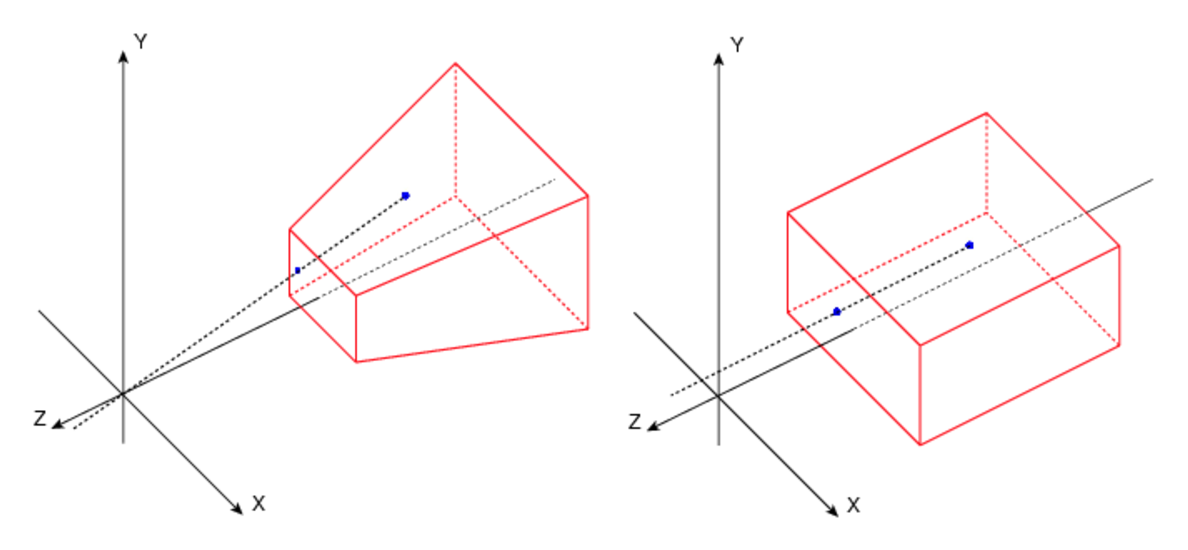
\includegraphics[width=0.6\textwidth]{graphics/perspective-orthographic.eps}
  \caption{Perspective (left) vs Orthographic (right)}
  \label{fig:perspective-orthographic}
\end{figure}
\FloatBarrier

\subsubsection{Orthographic}

Simple clip to a defined box defined by vertices $(left, bottom near)$ and
$(right, top, far)$.
\[
  P =
  \left [
    \begin{array}{cccc}
      \frac{2}{right - left}  & 0                       & 0                     & -\frac{right + left}{right - left} \\
      0                       & \frac{2}{top - bottom}  & 0                     & -\frac{top + bottom}{top - bottom} \\
      0                       & 0                       & \frac{2}{far - near}  & -\frac{far + near}{far - near} \\
      0                       & 0                       & 0                     & 1
    \end{array}
  \right ]
\]

Typically used for "flat" elements, e.g. menu, HUD, etc.

\subsubsection{Perspective}

Traditional perspective as perceived in real life.

\[
  P =
  \left [
    \begin{array}{cccc}
      \frac{f}{aspect}  & 0 & 0                             & 0 \\
      0                 & f & 0                             & 0 \\
      0                 & 0 & \frac{near + far}{near - far} & \frac{2 \cdot near \cdot far}{near - far} \\
      0                 & 0 & -1                            & 0
    \end{array}
  \right ]
\]

where:
\[
  f = \frac{1}{tan(fov / 2)}
\]

and $fov$ is the desired field of view.

\begin{description}
  \item[$x$ and $y$] \hfill \\
    Used to obtain distance along $x$ and $y$ axis with relation to $z$ and
    $fov$

  \item[$z$] \hfill \\
    Scale and translate $z$ position such that $z$ is in the range -1 to 1 after
    division by $w$

  \item[$w$] \hfill \\
    Set to $w = -1 \cdot z = -z$, this is used for the perspective divide

\end{description}

\subsubsection{Perspective Divide}

\url{https://www.khronos.org/opengl/wiki/Vertex_Post-Processing#Perspective_divide}

Have a vector $V$ for a vertex:
\[
  V =
  \left [
    \begin{array}{c}
      V_{x} \\
      V_{y} \\
      V_{z} \\
      w
    \end{array}
  \right ]
\]

Divide components of $V$ by $w$. This operation moves objects that are further
away (in $z$ axis) closer to the centre of the screen, this gives the effect of
a vanishing point.

\subsection{Object definition}

\[
  \left [
    \begin{array}{cccc}
      r_{xx}  & r_{xy}  & r_{xz}  & x \\
      r_{yx}  & r_{yy}  & r_{yz}  & y \\
      r_{zx}  & r_{zy}  & r_{zz}  & z \\
      0       & 0       & 0       & 1
    \end{array}
  \right ]
  \left [
    \begin{array}{c}
      V_{x} \\
      V_{y} \\
      V_{z} \\
      1
    \end{array}
  \right ]
\]

$(x, y, z)$ is the object position.

$r$ is the object orientation.

$(r_{xx}, r_{xy}, r_{xz})$ is the object left vector.

$(r_{yx}, r_{yy}, r_{yz})$ is the object up vector.

$(r_{zx}, r_{zy}, r_{zz})$ is the object facing vector.

The vertices of the object $V$ are transformed using the object matrix.

\subsection{MVP matrix}

Three stages of the standard transformation pipeline:

\begin{description}
  \item[Model] \hfill \\
    Local space to the world space

  \item[View] \hfill \\
    World space to camera space

  \item[Projection] \hfill \\
    Camera space to clip space

\end{description}

\section{Vertex/Geometry Operation}

\subsection{Amplification (Tessellation Shader)}

\url{https://www.khronos.org/opengl/wiki/Tessellation}

\begin{itemize}
  \item
    Tessellator runs after vertex shader

  \item
    Operates on patch primitives (generic $n$-sided primitive)

  \item
    Outputs tessellated geometry in either: triangles, quads or isolines

  \item
    Tessellation Control Shader is used to set tessellation level and perform
    any required patch transformations

    (Tessellation Control Shader is optional)

  \item
    Tessellation Evaluation Shader takes abstract coordinates generated by the
    tessellator and the patch coordinates and calculates the vertices of the
    output geometry

    (Tessellation Evaluation Shader is mandatory)

  \item
    Level of tessellation is set for inner and outer regions of tessellated
    geometry

    \begin{itemize}
      \item
        Inner level controls tessellation inside the area

      \item
        Outer level controls tessellation outside the area

      \item
        Edges that are shared between two tessellated areas must share the same
        outer tessellation level and vertex calculation to ensure continuity
        between areas
    \end{itemize}

\end{itemize}

TODO: diagrams

\subsection{Generation (Geometry Shader)}

\url{https://www.khronos.org/opengl/wiki/Geometry_Shader}

\begin{itemize}
  \item
    Geometry shader runs after tessellator

  \item
    Takes single primitive as input and outputs zero or more new primitives
    (limited types of primitives supported: points, lines \& triangles)

  \item
    Used to generate new (additional) geometry based on (limited) existing
    geometry

  \item
    e.g. basic graphical particle system in which points are sent to the GPU
    pipeline and are converted into quads by the geometry shader

    This saves (~75\%) CPU time copying primitives to the GPU

\end{itemize}

\subsection{Clipping}

\url{https://www.khronos.org/opengl/wiki/Vertex_Post-Processing#Clipping}

\begin{itemize}
  \item
    Remove geometry outside of viewing volume, reduced GPU load in rasterising
    (parts of) primitives that will never be seen

  \item
    Whole primitives that are outside viewing volume are simply culled as a
    whole

  \item
    Primitives that are partially outside are split at the boundary of the
    viewing volume and new primitives are created as needed to fill any space
    created inside the viewing volume (e.g. in the case of triangle clipping)

\end{itemize}

\subsection{Face Culling}

\url{https://www.khronos.org/opengl/wiki/Face_Culling}

\begin{itemize}
  \item
    Removes (culls) faces that will not be seen due to facing away from the
    camera

  \item
    Can cull front, back or all faces

    Culling all faces effectively disables the rasteriser for triangle based
    primitives

  \item
    Front and back faces are determined by the winding order of the vertices of
    triangles

\end{itemize}

\section{Fragment Operations}
\label{sec:fragment_operations}

\url{https://www.khronos.org/opengl/wiki/Per-Sample_Processing}

\subsection{Interpolation}

\Para{Lines}

Colour at point $p$ computed through simple linear interpolation between
vertices $v_{0}$ and $v_{1}$.
\begin{align*}
  C_{p} &= (C_{b} * t) + (C_{a} * (1 - t)) \\
  t &= |(v_{1} - p) / (v_{1} - v_{0})|
\end{align*}

\Para{Triangles}

Use Barycentric coordinates (section \ref{sec:barycentric}).
\[
  C_{p} = (\alpha * C_{a}) + (\beta * C_{b}) + (\gamma * C_{c})
\]

\subsection{Scissor testing}

\url{https://www.khronos.org/opengl/wiki/Scissor_Test}

\begin{itemize}
  \item
    Fragments outside of a given rectangle on the screen are discarded

  \item
    Can set unique scissor box per viewport
\end{itemize}

\subsection{Stencil testing}

\url{https://www.khronos.org/opengl/wiki/Stencil_Test}

\begin{itemize}
  \item
    Uses additional buffer attached to active framebuffer

  \item
    Each fragment has a stencil value

  \item
    Stencil value of a given fragment is tested against value in stencil buffer,
    if the test passes the fragment is used

  \item
    Operation on stencil buffer can be configured based on the result of the
    stencil and depth tests: keep current value, set to zero, invert current
    value, replace current value, increment, decrement, increment with wrap,
    decrement with wrap.

  \item
    Test is configurable: always, never, $=$, $\neq$, $<$, $\leq$, $>$, $\geq$

  \item
    Initial fragment stencil value is given for all fragments when configuring
    the stencil test

  \item
    Stencil testing can be performed on either front or back faces of a
    primitive, or both (state is held for both faces)

\end{itemize}

\subsection{Depth Buffer / Depth Test}

\url{https://www.khronos.org/opengl/wiki/Depth_Test}

Have a depth buffer which records the depth ($z$ coordinate) of the fragment
that has been rendered on a each pixel.

\begin{enumerate}
  \item[1]   When a pixel is to be shaded compare the $z$ coordinate of the new
    fragment with that in the depth buffer $D_{i}$
  \item[2.1] If $x \leq D_{i}$ then depth test passes, the pixel is shaded based
    on the new fragment and the depth buffer updated
  \item[2.1] Otherwise the test fails and the fragment is discarded
  \item[3]   The depth buffer is rest to maximum depth at the start of each
    frame
\end{enumerate}

Can have "z fighting" when two objects with close $z$ coordinates are rasterised
inside each other. A higher precision depth buffer avoids this.

\subsection{Blending}

\url{https://www.khronos.org/opengl/wiki/Blending}

Transparency denoted by alpha value in colour.

$\alpha = 1$ denotes full opacity, $\alpha = 0$ denotes full transparency.

Colour computed by blend equation:
\[
  C = (C_{source} * F_{source}) + (C_{dest} * F_{dest})
\]

Factors $F_{source}$ and $F_{dest}$ are usually programmable but a common
approach is standard linear blending:
\begin{align*}
  F_{source} &= \alpha \\
  F_{dest} &= 1 - \alpha
\end{align*}

One other alternative is additive blending:
\begin{align*}
  F_{source} &= 1 \\
  F_{dest} &= 1
\end{align*}

\section{Texture Mapping}

\begin{itemize}
  \item Texture coordinates $(u, v)$ defined per vertex
  \item Coordinated interpolated to obtain per fragment texture coordinates
  \item $(u, v)$ are normalised texture coordinates within $[0, 1]$
  \item Textures coordinates out of the $[0, 1]$ can be handled differently:
    \begin{description}
      \item[Clamp] \hfill \\
        Anything above 1 is set to 1 \\
        Anything below 0 is set to 0
      \item[Repeat] \hfill \\
        $1.1 = 0.1$ \\
        $-0.1 = 0.9$ \\
        etc.
      \item[Mirror] \hfill \\
        $1.1 = 0.9$ \\
        $-0.1 = 0.1$ \\
        etc.
    \end{description}
  \item All textures for a mesh typically stored in a single texture image
\end{itemize}

\subsection{Affine Transform}

Textures may not appear correctly if an object is tilted with respect to the
camera.

Caused by texture interpolation being linear but not fragment area.

Solution is to use affine transform:

\begin{enumerate}
  \item[1] Divide texture coordinates by $P_{w}$
  \item[2] Interpolate texture coordinates
  \item[3] Multiply by $P_{w}$
\end{enumerate}

\subsection{Bilinear Filtering}

When a texture is viewed close enough to the camera such that the rasterised
object takes up more pixel space than the texture image.

Sample multiple texels and blend them together.

e.g. for texel coordinate 7.6 blend colour of texel 7 and 8 by factor 0.6.

\subsection{MIP mapping /  minification}

Generating smaller textures using the original fill size texture so that objects
further away can sample a smaller texture.

Forms a set of textures in decrecing size, known as a MIP chain.

MIP map is selected using the level of detail (LOD) $\lambda$.

This is calculated using the derivatives of the interpolated $x$ and $y$
texture coordinates, i.e. how fast the texture coordinates are changing.

Faster change in texture coordinates (higher $\lambda$) means less unique texels
hence less detail. The size of $\lambda$ denotes how far down the MIP change the
texture is selected.

MIP chain is pre processed when the texture is loaded.

Requires more memory to store entire MIP chain opposed to a single texture, but
gives faster processing as less work needs to be done during rasterisation and
gives a better texture quality due to texel averaging.

\subsubsection{Trilinear filtering}

Similar to bilinear filtering (operating in $x$ and $y$ axes) but also operating
in $z$ axis to interpolate between two MIP map levels.

Solves issue when an object spans multiple MIP levels and a noticeable line where
the texture quality changes can be seen.

\section{Scene Hierarchy and Skeletal animation}

\subsection{Scene Graphs}

\begin{itemize}
  \item Hierarchical tree structure of meshes
  \item Each mesh has a model matrix that gets applied to it and all its
    children
  \item Typically use a tree as shallow as possible to reduce traversal time
  \item Can include many other (non graphical) objects on the tree:
    \begin{itemize}
      \item Sound emitters
      \item Shaders
      \item etc.
    \end{itemize}
\end{itemize}

Need to ensure transparent objects are drawn in the correct order. Solution is
to add a "transparency" tag to each node.

When processing objects:
\begin{enumerate}
  \item[1] Traverse the tree and build a list of opaque objects and a list of
    transparent objects
  \item[2] Render all the opaque objects
  \item[3] Sort the list of transparent objects by their $z$ position
  \item[4] Render transparent object from furthest away to closest
\end{enumerate}

\subsection{Animation}

Can do simple animation by manipulating a tree of objects and their model
matrices. This works well for simple objects such as cars and robots.

It will not work for objects that have a flexible skin (such as humans).

\subsubsection{Skinned meshes}

Instead a skinned mesh is used and each vertex is pulled in the direction of
several skeletal nodes (joints) by a set of weights.

Skeletal nodes are arranged in a hierarchical tree and inherit transformations.

Skinning (the process of transforming vertices of the mesh based on weights) is
typically done on the vertex shader. An array of transformations can be passed
to the shader through a uniform.

The assignment of weights to each vertex and node (rigging) is done offline in
the 3D modelling suite.

In order to get a good frame rate in a skeletal animation without having to
reskin the mesh every frame animation can be interpolated.

In order to combine multiple animations that affect different parts of the
skeleton, different animations can be blended together to form a new animation.

Joints can usually be queried to obtain the transformation, useful when
attaching other meshes to them (e.g. attach a gun to a hand).

Inverse kinematics can be used to position a child node in a given position and
have the parent nodes move in a realistic manner (e.g. placing a hand on a door
handle).

\section{Lighting}

\subsection{Normals}

\begin{itemize}
  \item Unit vector perpendicular to the surface
  \item Can be calculated using cross product of two side vectors
  \item Usually stored as part of the model
  \item Vertex normals are interpolated across the primitive
  \item Interpolation may cause problems if an object has sharp corners
\end{itemize}

\subsection{Lighting Models}

\begin{description}
  \item[Static lighting] \hfill \\
    Combining texture with a light map. \\
    No real time updates. \\
    No additional computation.

  \item[Flat shading] \hfill \\
    Per surface lighting. \\
    Single value used on a surface. \\
    Computationally fast.

  \item[Gourard shading] \hfill \\
    Per vertex shading. \\
    Interpolated across primitive. \\
    More computationally expensive.

  \item[Phong shading] \hfill \\
    Per fragment lighting. \\
    Most computationally intensive.

  \item[Bump Mapping] \hfill \\
    Normals stored in texture. \\
    Each texel has its own normal.

\end{description}

\subsection{Phong Reflection Model}

Types of light:

\begin{description}
  \item[Ambient] \hfill \\
    Lights all faces of all objects in a scene equally
  \item[Diffuse] \hfill \\
    Light from a source that has been scattered evenly
  \item[Specular] \hfill \\
    Light from a source that has been reflected towards the camera
\end{description}

Lighting colour $c$ of a fragment (for a single light):
\begin{align*}
  c &= c_{a} + (c_{d} + c_{s}) \times a \\
  c_{d} &= (N \cdot |(L - P)|) \times C_{d} \\
  c_{s} &= (N \cdot \frac{1}{2}(V + L))^{n} \times C_{s}\\
  a &= 1 - \frac{L}{L_{max}}
\end{align*}

where:

\begin{itemize}
  \item $k_{a}$ is the constant ambient light for the scene
  \item $L_{max}$ is the maximum distance that a light source can be away from a
    source
  \item $L$ is the distance from the light source to the surface
  \item $n$ is the specular power (higher for shinier materials)
  \item $C_{d}$ and $C_{s}$ are colours of the diffuse and specular light
  \item $P$ is the fragment position
  \item $V$ is the view vector
  \item $L$ is the light vector
  \item $N$ is the normal
\end{itemize}

Normal $N$ can be calculated using two side vectors: $N = (v_{0} - v_{1}) \times
(v_{0} - v_{2})$

Attenuation factor $a$ ensures that the light gets weaker as the light source
moves away from the surface.

\subsection{Shadow mapping}

TODO

\section{Post processing}

TODO

\section{Deferred Rendering}

TODO

\end{document}
